%Every LaTeX file needs a documentclass declaration.
%Possibilities are article, book, letter.  Font size is also declared.

\documentclass[10pt]{article}

%special packages used for symbols, formatting, etc.

\usepackage{amsmath} % contains the align* environment, which is great for manipulating formulas
\usepackage{amssymb} % contains common symbols
\usepackage{amsthm} % has the proof environment
\usepackage[margin=1in]{geometry} % specifies page properties, such as the margin
%\usepackage{siunitx} % useful for typesetting units
\usepackage{xcolor}
\usepackage{graphicx}

% User-defined commands

\newcommand{\newprob}{\medskip \hrule \medskip}
\newcommand{\fanc}[1]{\mathbb{#1}}
\newcommand{\rn}[1]{\fanc{R}^{#1}}
\def\qed{\hspace*{\fill}\rule{1.854mm}{3mm}}  % the fancy box at the end of a proof

%%%%%%%%%%%%%%%%%%%%%%%%%%%%%%%%%%%%%%%%%%%%%%

%beginning of document, every \begin{} also requires an \end{} command.

%\renewcommand{\baselinestretch}{2}

\begin{document}

\pagestyle{empty}  %suppress page numbers, etc.

\begin{center}  %center command, also see flushright, flushleft

{\bf MATH 423-01  Advanced Calculus I

Homework \# 1

Assigned: August 29, 2022

Due: September 7, 2022}

\end{center}

\medskip

\hrule   %horizontal line

\bigskip

% list environment: description, itemize, and enumerate

\begin{enumerate}

%%%%%%%%%%%%%%%%%%%%%%

\item  ~[Aitchison, A.] State the contrapositive ($\neg q \to \neg p)$ of each of the following conditional statements.  It will help in some cases to rewrite the statement as $p \to q$ before starting.

	\begin{enumerate}
	
	\item  If it snows today, then I will ski tomorrow.
  \par \medskip
 \textbf{\textcolor{black}{\underline{Answer}:}}
{\textcolor{black}{If it doesn't snow today, then I will not ski tomorrow.}}
	
	\item  I come to class whenever there is going to be a quiz.
  \par \medskip
  \textbf{\textcolor{black}{\underline{Answer}:}}
{\textcolor{black}{If there is not going to be a quiz, then I will not go to class.}}
	
	\item  A positive number is a prime only if it has no divisors other than $1$ and itself.
	  \par \medskip
  \textbf{\textcolor{black}{\underline{Answer}:}}
{\textcolor{black}{If a positive number does have divisors other than 1 and itself, then it is not prime.}}
	\item  I go to the beach whenever it is a sunny summer day.
	   \par \medskip
  \textbf{\textcolor{black}{\underline{Answer}:}}
{\textcolor{black}{If it is not a sunny summer day, then I do not go to the beach.}}
	\item  When I stay up late, it is necessary that I sleep until noon.
		   \par \medskip
  \textbf{\textcolor{black}{\underline{Answer}:}}
{\textcolor{black}{If I stay up late, then it is necessary for me to sleep till noon.}}
	
	\end{enumerate}

\item  ~[Delfosse, D.] Describe what we would have to demonstrate in order to disprove each of the following statements.

	\begin{enumerate}
	
	\item  At every college in the United States there is a student who is at least seven feet tall.
 	 \par \medskip
  \textbf{\textcolor{black}{\underline{Answer}:}}
{\textcolor{black}{To disprove this example, we would need to find a college in the United States where every student is less than seven feet tall.}}
	
	\item  For all colleges in the United States, there exists a professor who gives every student a grade of either A or B.
 	\par \medskip
  \textbf{\textcolor{black}{\underline{Answer}:}}
{\textcolor{black}{To disprove this example, we would need to find a college in the United States where all professors give grades other than A's or B's.}}
	
	\item  There exists a college in the United States where every student is at least six feet tall.
 	 \par \medskip
  \textbf{\textcolor{black}{\underline{Answer}:}}
{\textcolor{black}{To disprove this example, we would need to show that there is a student who is less than six feet tall at every college in the United States.}}
	
	\end{enumerate}

\item\label{prob:DeMorgan}  Prove De Morgan's Laws.  Assume that $A$ and $B$ are sets.

	\begin{enumerate}
	
	\item  ~[Griffith, B.] $\left( A \cap B \right)^{c} = A^{c} \cup B^{c}$.
\begin{proof}
{\textcolor{black}{Assume A and B are sets. $(\subseteq)$ Suppose that $x \in \left( A \cap B \right)^{c}$.  This means that $x \notin (A \cap B)$.  Since the intersection is the set of all elements common to both A and B, the previous step means that $x \notin A $ and B.  This means that $x \in A^C$ or $x \in B^C$.  By definition, this means that $x \in A^C \cup B^C$. $(\supseteq)$ Suppose that $x \in A^C \cup B^C$.  This means that $x \in A^C$ or $x \in B^C$.  Thus, $x \notin A$ or B.  So, $x \in (A \cap B)^C$. Therefore, $\left( A \cap B \right)^{c} = A^{c} \cup B^{c}$.}}
\end{proof}

 
	\item  ~[Hale, A.] $\left( A \cup B \right)^{c} = A^{c} \cap B^{c}$.
  \begin{proof}
\textcolor{black}{Assume A and B are sets. $(\subseteq)$ Suppose that $x \in \left( A \cup B \right)^{c}$.  This means that $x \notin (A \cup B)$. So, $x \notin A$ and $x \notin$ B. According to the definition of complement, $x \in A^C$ and $x \in B^C$.  Therefore, $x \in A^C \cap B^C$. $(\supseteq)$ Suppose that $A^{c} \cap B^{c}$.  This means that $x \in A^C$ and $x \in B^C$.  This means that $x \notin A$ and $x \notin B$, which means $x \notin (A \cap B)$.  Since this statement is true, then $x \in (A \cup B)^C$.  Therefore, $\left( A \cup B \right)^{c} = A^{c} \cap B^{c}$.}
\end{proof}
	
	\end{enumerate}
	
\item\label{prob:identities}  Let $A$, $B$, and $C$ be sets.  Prove the following statements.

	\begin{enumerate}
	
	\item  ~[Powers, S.] $A \cup (B \setminus A) = A \cup B$.
\begin{proof}
Let A, B, and C be sets.  Let $x \in A \cup (B \backslash A)$.  Then $x \in A$ or $x \in (B \backslash A)$ by definition of union.  So, $x \in B$ and $x \notin A$ (by set difference).  But $x \in A$ by previous statement, so $x \in A$ or $x \in B$.  By definition of union, $x \in (A \cap B)$.  Thus, $A \cup (B \setminus A) = A \cup B$.
\end{proof}
	\item  ~[Schipke, K.] $A \cap (B \setminus A) = \emptyset$.
 \begin{proof}
Let A, B, and C be sets.  Assume $A \cap (B \backslash A) \neq \emptyset$.  Let $x \in A \cap (B \backslash A)$.  This means $x \in A$ and $x \in (B \backslash A)$.  So, $x \in A$ and $(x \in B$ and $x \notin A)$.  But this is a contradiction, since it cannot be the case that $x \in A$ and $x \notin A$.  Therefore, since the assumption that $A \cap (B \backslash A) \neq \emptyset$ leads to a contradiction, it follows that $A \cap (B \setminus A) = \emptyset$.
\end{proof}
	\item  ~[Schmidt, S.] $(B \setminus A) \cup (C \setminus A) = (B \cup C) \setminus A$.
 \begin{proof}
Let A, B, and C be sets.  Let $x \in (B \backslash A) \cup (C \backslash A)$.  Then $x \in (b \backslash A)$ or $x \in (C \backslash A)$.  If $x \in (B \backslash A)$, then $x \in B$ and $x \notin A$ by definition of set difference.  If $x \in (C \backslash A)$, then $x \in C$ and $x \notin A$.  By definition of union, $x \in (B \cup C)$ and $x \notin A$, then $x \in (B \cup C)\backslash A$.  Thus, $(B \setminus A) \cup (C \setminus A) = (B \cup C) \setminus A$.   
 \end{proof}
	\item  ~[Smith, G.] $A \setminus B = A \cap B^c$.
\begin{proof}
We must show two cases: $A \backslash B \subseteq A \cap B^C$ and $A \cap B^C \subseteq A \backslash B$.  First, prove $A \backslash B \subseteq A \cap B^C$.  Let $x \in A \backslash B$.  By definition of set difference, $x \in A$ and $x \notin B$.  By definition of complement, $x \notin B$ implies that $x \in B^C$.  Hence, it is true that both, $x \in A$ and $x \in B^C$.  By definition of intersection, $x \in A \cap B^C$.  Then, prove $A \cap B^C \subseteq A \backslash B$.  Let $x \in A \cap B^C$.  By definition of intersection, $x \in A$ and $x \in B^C$.  By definition of complement, $x \in B^C$ implies that $x \notin B$.  Hence, $x \in A$ and $x \notin B$.  By definition of set difference, $x \in A \backslash B$.  Thus, $A \setminus B = A \cap B^c$.
\end{proof}
	\item  ~[Wright, A.] $(A \cap B) \cup (A \cap B^c) = A$.
 \begin{proof}
Let A, B, and C be sets.  We must prove equality by double containment.  $(\subseteq)$ Let $x \in (A \cap B) \cup (A \cap B^C).$  Then either $x \in A \cap B$ or $x \in A \cap B^C$.  In either of those two cases, we must have $x \in A$ by definition of intersection.  Therefore, $(A \cap B) \cup (A \cap B^C \subseteq A$.  $(\supseteq)$ Let $x \in A$.  Then either $x \in B$ or $x \in A \cap B^C$.  By definition of union, we therefore have $x \in (A \cap B) \cup (A \cap B^C)$.  Thus, $(A \cap B) \cup (A \cap B^C) \supseteq A$.  Therefore, $(A \cap B) \cup (A \cap B^c) = A$.
 \end{proof}
	
	\end{enumerate}
	
\item\label{prob:sym_diff}  ~[Deschamp, B.] The \emph{symmetric difference} of the sets $A$ and $B$, denoted $A \oplus B$, is the set containing those elements in either $A$ or $B$ but not in both $A$ and $B$.  In class we showed that \begin{equation}\label{eq:sym_diff} A \oplus B = (A \cup B) \setminus (A \cap B) = (A \setminus B) \cup (B \setminus A).\end{equation}  Prove that $(A \oplus B) \oplus B = A$.

\textbf{This is a different type of set argument.  It would be too complicated to write a proof using elements of these sets.  Instead of an element-wise argument, this problem works better with a set-wise argument.  In this case the idea is to use the identities in Problems \ref{prob:DeMorgan} and \ref{prob:identities} to write out one side of $A \oplus B$ given in (\ref{eq:sym_diff}) and then use various identities to manipulate one side of the equation into the other side of (\ref{eq:sym_diff}).  At each stage of the manipulation state which identity you used.  I needed the following additional identities.  If you invent your own identity, give it a unused letter and make sure that you provide proof that the identity is true.}

	\begin{center}
	\begin{tabular}{l@{\hspace{0.4in}}l@{\hspace{0.5in}}l}
	(a) $A \setminus (B \cup C) = (A \setminus B) \cap (A \setminus C)$ & (b) $B \setminus (A \cap B^c) = B$ & (c) $B \setminus (B \cap A^c) = A \cap B$\\
	\end{tabular}
	\end{center}
 \begin{proof}
One way to conduct this proof besides Deschamp's way is to use a truth table to cover all the cases.
\par \medskip
 \begin{figure}[!ht]
\centering  %centering can be used to center the image
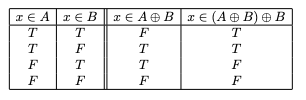
\includegraphics[height=25mm]{Homeworks/Homework 1/Prob 5 Truth Table.png}
 \caption{Truth Table for $(A \oplus B) \oplus B = A$}
 \label{f:Chart 1}
\end{figure}
Since the column under $A$ and the column under $(A \oplus B) \oplus B$, are the same, then the two sets are equal.  Therefore, $(A \oplus B) \oplus B = A$.
 \end{proof}
	
% This is a future problem for a future assignment.  Don't worry about this problem.	
	
%\item  Use the Triangle Inequality to prove the following inequalities.
%
%	\begin{enumerate}
%	
%	\item  $|a-b| \leq |a| + |b|$.  Hint: hide the negative sign inside a substitution.
%	
%	\item  $||a| - |b|| \leq |a-b|$.  Hint: split this into two cases, (i) $|a| - |b| \leq |a-b|$ and (ii) $-(|a| - |b|) \leq |a-b|$.  For (i) try to prove that $|a| \leq |b| + |a-b|$.
%	
%	\end{enumerate}

\newpage

\item  ~[Papiernik, J.] Consider a set $A$.  The \emph{power set} of $A$, denoted $\mathcal{P}(A)$, is the set that contains all of the subsets of $A$.  For example, if $A = \{ 1, 2 \}$, then $\mathcal{P}(A) = \{ \emptyset, \{1\}, \{2\}, \{1,2\} \}$.  Prove that $|\mathcal{P}(A)| = 2^n$, where $|A| = n$.  Hint: use a counting argument.
\begin{proof}
We know that $_n C_r = \frac{n!}{r!(n-r)!}!$ and $(a+x)^n = _n C_0*a^n*x^0+_n C_1*a^{n-1}x^1 \cdots$.  Let A be a set, where $|A| = n$.  So, 
\begin{center}
\par \medskip
-Subset with 0 elements = $_n C_0$
\par \medskip
-Subset with 1 element = $_n C_1$
\par \medskip
-Subset with 2 elements = $_n C_2$
\par \medskip
$\cdots$
\par \medskip
-Subset with n elements = $_n C_n$
\par \medskip
\end{center}
Therefore, the total subset = $_n C_0 + _n C_1 + _n C_2 + \cdots + _n C_n$.  We know that $(a+x)^n = _n C_0*a^n*x^0+_n C_1*a^{n-1}x^1 \cdots + _n C_n*a^0*x^n$.  If we substitute $a = 1$ and $x = 1$, we get the following equation: 
\begin{center}
\par \medskip
    $(1+1)^n = _n C_0*1^n*1^0+_n C_1*1^{n-1}1^1 + _n C_2*1^{n-2}1^2 \cdots +  _n C_n*1^0*1^n$
    \par \medskip
    $2^n = _n C_0 + _n C_1 + _n C_2 + \cdots _n C_n$
    \par \medskip
\end{center}
Therefore, $|\mathcal{P}(A)| = 2^n$, where $|A| = n$.
\end{proof}

\item  Recall that given a function $f:A \to B$ the \emph{range} of $f$ is the set $\{ y \in B: y=f(x) \textnormal{ for some } x \in A\}$.  Note that the range is a subset of the codomain, but they may not be equal.  Let $S$ be a subset of the domain $A$.  The \emph{image} of $S$ is the set $f(S) = \{f(x): x \in S \}$.  Note that this means the range is the image of the domain.

Let $f:A \to B$, and let $S$ and $T$ be subsets of $A$.

	\begin{enumerate}
	
	\item  ~[Lindskov, I.] Prove that $f(S \cup T) = f(S) \cup f(T)$.
 \begin{proof}
Given that $f A\rightarrow B$ is a function and S and T are subsets of A, then $f(S)$ and $f(T)$ are in $f(A)$.  Two cases must be proven. 
  In the first case, let $b \in f(S \cup T)$.  Then $b = f(a)$ for some $a \in S \cup T$.  So $a \in S$, $a \in T$, or is in both.  Because of this, then $f(a) \in f(s)$ or $f(a) \in f(T)$ and $b \in f(S)$ or $b \in f(T)$.  By the definition of union, then $b \in f(S) \cup f(T)$.  So $f(S \cup T) \subseteq f(S) \cup f(T)$.  Then to prove the other case, let $b \in f(S) \cup f(T)$.  Then $b \in f(S)$, $b \in f(T)$, or in both.  This means that $b = f(a)$ for some $a \in S$, $a \in T$, or both.  Because of this, then $b \in f(S \cup T)$.  Thus, $f(S) \cup f(T) \subseteq f(S \cup T)$.  From these two cases, we can conclude that $f(S \cup T) = f(S) \cup f(T)$.
 \end{proof}
	\item  ~[Nupen, R.] Prove that $f(S \cap T) \subseteq f(S) \cap f(T)$.
\begin{proof}
Let $b \in f(S \cap T)$. Then $b = f(a)$ for some element $a \in S \cap T$.  Since $a \in S$, $a \in T$, or in both, then $f(a) \in f(S), f(T)$, or in both.  So, $b \in f(S) \cap f(T)$.  Thus, $f(S \cap T) \subseteq f(S) \cap f(T)$.
\end{proof}
    
	\item  ~[Nupen, R.] Find a function and two sets for which $f(S \cap T) \neq f(S) \cap f(T)$.
	
	\textbf{For this counterexample I recommend what is sometimes called a toy example.  This means finding a very simple example with very small sets (maybe just a number or two in the set) and a very simple function.  To make this work, find $S$ and $T$ such that $S \cap T = \emptyset$.  This isn't required, but it will make things easier.  The key is to find a function that is not injective.  For those of you who want to get at the heart for why the backward containment ($\supseteq$) fails, try to prove that direction and note where the function $f$ has to be injective for things to work.}
 \par \medskip
  \textbf{\textcolor{black}{\underline{Answer}:}}
{\textcolor{black}{Define $f: \mathbb{R} \rightarrow \mathbb{R}$ as $f(x) = x^2$.  Let $S = [-1, 0]$ and $T = [0,1]$.  Then, $f(S) = [0,1]$ and $f(T) = [0,1]$.  Therefore $f(S) \cap f(T) = [0,1]$.  But, $S \cap T = \{0\}$, therefore, $f(S \cap T) = \{0\}$.  Clearly, $f(S \cap T) \neq f(S) \cap f(T)$.}}
	
	\end{enumerate}
	
\item  Given a function $f: D \to \mathbb{R}$ and a subset $B \subseteq \mathbb{R}$, let $f^{-1}(B)$ be the set of all numbers from the domain $D$ that are mapped into $B$; that is, $f^{-1}(B) = \{ x \in D: f(x) \in B \}$.  Note that this is a set of numbers and not an inverse function.  This set is called the \emph{preimage} of $B$.

	\begin{enumerate}
	
	\item  ~[Kline, L.] Let $f(x) = x^2$.  If $A$ is the closed interval $[0,4]$ and $B$ is the closed interval $[-1,1]$, find $f^{-1}(A)$ and $f^{-1}(B)$.  Is it true that $f^{-1}(A \cap B) = f^{-1}(A) \cap f^{-1}(B)$ and $f^{-1}(A \cup B) = f^{-1}(A) \cup f^{-1}(B)$?
  \begin{proof}
If $x \in [-2,2]$, then it is certainly true that $f(x) \in A$.  Moreover, these are the only possible values of x such that $f(x) \in A$, so we can see that $f^{-1}(A) = [-2,2]$.  Turning to B, notice that, if $x \in [-1,1]$, then $f(x) \in B$ and, in fact, these are the only real numbers that map to B under f (of course, there is no real number x such that $f(x) < 0$, so half of B is completely missed by f). Therefore, $f^{-1}(B) = [-1,1]$ (which is, coincidentally, B again, so $f^{-1}(B) = B$).  Now $A \cap B = [0,4] \cap [-1,1] = [0,1]$ and $f^{-1}([0,1])=[-1,1]$, so we see that $f^{-1}(A \cap B) = [-1,1]=[-2,2] \cap [-1,1] = f^{-1}(A) \cap f^{-1}(B)$.  On the other hand, $a \cup B = [-1, 4]$ and $f^{-1}([-1,4]) = [-2,2]$, so we also have that $f^{-1}(A \cup B) = [-2,2]=[-2,2] \cup [-1,1] = f^{-1}(A) \cup f^{-1}(B)$.
 \end{proof}
	\item  ~[Kline, L.] Show that for an arbitrary function $g: \mathbb{R} \to \mathbb{R}$ that $g^{-1}(A \cap B) = g^{-1}(A) \cap g^{-1}(B)$.
\begin{proof}
First, we want to show that $g^{-1}(A \cap B) = g^{-1}(A) \cap g^{-1}(B)$. To do this, we must show inclusion in two ways.  To show that $g^{-1}(A \cap B) \subseteq g^{-1}(A) \cap g^{-1}(B)$, suppose that $x \in g^{-1}(A \cap B)$.  By definition, this means that $g(x) \in A \cap B$.  In particular, this means that $g(x) \in A$ and $g(x) \in B$ or, equivalently, $x \in g^{-1}(A)$ and $x \in g^{-1}(B)$.  This means that $x \in g^{-1}(A) \cap g^{-1}(B)$.  Then $x \in g^{-1}(A)$ and $x \in g^{-1}(B)$ and so, by definition, this means that $g(x) \in A \cap B$, which implies that $x \in g^{-1}(A \cap B$.  Since our choice of $x$ was arbitrary, we can conclude that $g^{-1}(A) \cap g^{-1}(B) \subseteq g^{-1}(A \cap B)$.  Having shown inclusion both ways, we can conclude that $g^{-1}(A \cap B) = g^{-1}(A) \cap g^{-1}(B)$.
\end{proof}
	\item  ~[Krason, T.] Show that for an arbitrary function $g: \mathbb{R} \to \mathbb{R}$ that $g^{-1}(A \cup B) = g^{-1}(A) \cup g^{-1}(B)$.
\begin{proof}
Now, we want to show that $g^{-1}(A \cup B)= g^{-1}(A)\cup g^{-1}(B)$. Following the usual pattern, we want to show first that $g^{-1}(A \cup B) \subseteq g^{-1}(A) \cup g^{-1}(B)$, so suppose that $x \in g^{-1}(A \cup B)$. By definition, this means that $g(x)\in A \cup B$, so $g(x)\in A$ or $g(x)\in B$. Stated equivalently, $x \in g^{-1}(A)$ or $x \in g^{-1}(B)$, which implies that $x \in g^{-1}(A) \cup g^{-1}(B)$. Since our choice of $x$ was arbitrary, we see that $g^{-1}(A \cup B) \subseteq g^{-1}(A) \cup g^{-1}(B)$.  To show the other inclusion, suppose $x \in g^{-1}(A) \cup g^{-1}(B)$. This means that $x \in g^{-1}(A)$ or $x \in g^{-1}(B)$, which is to say that $g(x)\in A$ or $g(x) \in B$. Either way, $g(x) \in A \cup B$, and so $x \in g^{-1}(A \cup B)$. Since the choice of $x$ was arbitrary, we see that $g^{-1}(A) \cup g^{-1}(B) \subseteq g^{-1}(A \cup B)$.Having shown both inclusions, we can conclude that $g^{-1}(A \cup B)= g^{-1}(A)\cup g^{-1}(B)$, as desired.
\end{proof}
	\end{enumerate}
	
\item  Assume that De Morgan's Laws in Problem \ref{prob:DeMorgan} have been proven.  Assume that $A_1, A_2, \ldots, A_n$ are sets.

	\begin{enumerate}
	
	\item  ~[Harter, J.] Use induction to prove that $$\left( A_1 \cup A_2 \cup \cdots \cup A_n \right)^c = A_1^c \cap A_2^c \cap \cdots \cap A_n^c.$$
 \begin{proof}
Let $P(n)$ be the statement that $(A_1 \cup A_2 \cup \cdots \cup A_n)^c = A_1^c \cap A_2^c \cap \cdots \cap A_n^c$.  To prove this, we must use induction.  For the base case, we must assign $n = 2$.  Then, we have by DeMorgan's Law, $(A_1 \cup A_2)^c = (A_1)^{c} \cap (A_2)^c$.  Because of this fact, then $P(2)$ is true.  For the inductive step, let $P(n)$ be true for $n = k$ i.e. $(A_1 \cup A_2 \cup \cdots \cup A_k)^c = A_1^c \cap A_2^c \cap \cdots \cap A_k^c$.  For $n = k+1$, we have $(A_1 \cup A_2 \cup \cdots \cup A_{k+1})^c = [(A_1^c \cup A_2^c \cup \cdots \cup A_{k}) \cup A_{k+1}]^c = (A_1 \cup A_2 \cup \cdots \cup A_k)^c \cap A_{k+1}^c = ((A_1)^c \cap (A_2)^c \cap \cdots (A_k)^c) \cap (A_{k+1})^c = (A_1)^c \cap (A_2)^c \cap \cdots \cap (A_{k+1})^c$.  Therefore, $P(n)$ is true for $n = k+1$.  Hence, by induction, we can say that $P(n)$ is true for all $n$.
 \end{proof}
	
	\item  ~[Harter, J.] Explain why induction cannot be used to conclude that $$\left( \bigcup_{k=1}^{\infty} A_k \right)^c  = \bigcap_{k=1}^{\infty} A_k^c.$$
 \par \medskip
	\textbf{\textcolor{black}{\underline{Answer}:}}
{\textcolor{black}{We cannot use the induction method to prove this because the induction method says that if a statement is true for n = 1, then we assume it is true for n = k and then prove that n = k + 1 is true as well.  In this case, the sets are infinite, so we cannot say anything about the sets and if they have intersection to each other or not.  Maybe given the hypothesis is true for  n = k and n = k+1, but still we cannot say more than that.  Hence, induction would not be the correct way to prove this statement.}}
	
	\item  ~[James, J.] Is the above statement true?  If not, provide a counterexample.  If it is true, prove the statement without using induction.
 \par \medskip
	\textbf{\textcolor{black}{\underline{Answer}:}}
{\textcolor{black}{The statement above is true.}}
\begin{proof}
Let $x$ be a set in either subsets $A_k \subset x$ for $k = 1, \cdots, \infty$.  Let $(\bigcup_{k=1}^{\infty} A_k)^c = S$ and $\bigcap_{k=1}^{\infty} A_k^c = T$.  To establish the equality, $S = T$, we will show that $S \subset T$ and $T \subset S$.  Let $x \in S$.  Then $x \in (\bigcup_{k=1}^{\infty} A_k)^c$.  This means that $x \notin A_k$ for any $k$.  Then $x \in A_k^c \forall k = 1, \cdots, \infty$.  Then $x \in \bigcap_{k=1}^{\infty} A_k^c$.  Which means that $x \in T$.  Therefore, $S \subset T$.  Conversely, let $x \in T = \bigcap_{k=1}^{\infty} A_k^c$.  Which means that $x \in A_k^c \forall k = 1, \cdots,\infty$ for some $k$.  So, $x \notin A_k$, and $x \notin (\bigcup_{k=1}^{\infty} A_k)$.  Thus, $x \in (\bigcup_{k=1}^{\infty} A_k)^c$ and $x \in S$.  Therefore, $T \subset S$.  From the two cases, we can conclude that $(\bigcup_{k=1}^{\infty} A_k)^c = \bigcap_{k=1}^{\infty} A_k^c$.
\end{proof}
	
	\end{enumerate}
	
\newpage
	
\item  ~[Staat, E.]  A function, $f$,  whose domain and codomain are subsets of $\mathbb{R}$ is called \emph{increasing} if $f(x) \leq f(y)$ whenever $x < y$ and $x$ and $y$ are in the domain of $f$.  A function, $f$,  whose domain and codomain are subsets of $\mathbb{R}$ is called \emph{strictly increasing} if $f(x) < f(y)$ whenever $x < y$ and $x$ and $y$ are in the domain of $f$.

	\begin{enumerate}
	
	\item  Prove that a strictly increasing function from $\mathbb{R}$ to $\mathbb{R}$ is injective.  Hint: note that the definition of an injective function deals with numbers being equal.  In this problem we don't anything that would help us show that numbers are equal, since we're only given inequalities.  As a result, use the contrapositive of the definition of an injective function.  Be careful, I'm not suggesting a proof by contrapositive, only that you use the contrapositive of the definition.
 \begin{proof}
     If $x \neq y$, then either $x < y$ or $y < x$.  In the first case, we have $f(x) < f(y)$, and in the second case, we have $f(y) < f(x)$.  In both cases, we have $f(x) \neq f(y)$, and by definition, it means that $f$ is injective.
 \end{proof}
	
	\item  Give an example of an increasing function from $\mathbb{R}$ to $\mathbb{R}$ that is not injective.
 \par \medskip
	\textbf{\textcolor{black}{\underline{Answer}:}}
{\textcolor{black}{One example of an increasing function from $\mathbb{R}$ to $\mathbb{R}$ that is not injective is one that's graph continues on indefinitely up and to the right and down and to the left.  After experimenting, one way to show this algebraically is the function $x^3-x$.  The reason this function works is that every horizontal line meets the graph somewhere.  It is not injective since some horizontal lines meet the graph at more than one point.}}
	\end{enumerate}
	
\item  Suppose that $g: A \to B$ and $f:B \to C$.  Recall that the \emph{composition} $f \circ g: A \to C$ is the function $(f \circ g)(x) = f(g(x))$.

	\begin{enumerate}
	
		\item  {~[Lauen, A.] Show that if both $f$ and $g$ are injective, then $f \circ g$ is also injective.}
\begin{proof}
Let $A$, $B$, and $C$ be sets.  Also, let $f: B \xrightarrow{} C$ and $g:  A\xrightarrow{} B$ be functions.  Let $f$ and $g$ be injective.  This means that given values $f(a) \in C$ and $f(b) \in C$ with $f(a)=f(b)$, then $a = b$.  This also means that given values $g(m) \in B$ and $g(n) \in B$ with $g(m)=g(n)$, then $m = n$.  Assume $(f \circ g)(x) = (f \circ g)(y)$.  This statement can be rewritten as $f(g(x)) = f(g(y))$ given the definition from the problem.  Then call $a = g(x)$ and $b = g(y)$.  After this call, then it can be said that $f(a) = f(b)$.  Because $f$ is injective, then $a=b$.  Since $a = b$, it can be rewritten as $g(x) = g(y)$ from above.  Because g is injective, it can be said that $x=y$.  Therefore $f \circ g$ is injective.

%Then, $f(a)=g(b)$.  Because of these definitions, it can be attempted to compose them.  This would be $f(g(a)) = f(g(b))$ by definition of injection.  After doing this computation, it can be determined that $(f \circ g)$ is injective.
 \end{proof}
	\item  ~[Lewis, J.] Show that if both $f$ and $g$ are surjective, then $f \circ g$ is also surjective.
\begin{proof}
Let $A$, $B$, and $C$ be sets. Let $f: B \xrightarrow{} C$ and $g: A \xrightarrow{} B$ be functions. Let $f$ and $g$ be surjective. This means that given the value $a \in C$, then there exists a $b \in B$ such that $f(b) = a$.  This also means that given value $m \in B$, there exists a $n \in A$ such that $g(m) = n$.  Assume there exists a value $y \in C$.  Since $f$ is surjective, then there exists a $x \in B$ such that $f(x) = y$ since B is the domain of $f$. Because $g$ is surjective and its codomain is B, then there exists a $y \in A$ such that $g(x) = y$.  Therefore $f \circ g$ is surjective.

% This can be rewritten as $f(g(x)) = y$, given the definition from the problem.  
% Then, call $a = y$ and $b = g(x)$.  After this call, it can be said that there exists an $a \in C$. Because $f$ is surjective, then $f(b) = a$. Since, $f(b) = a$, it can be written as $f(x) = y$ from above.  Because $g$ is surjective, it can be said that $g(x) = y$. Therefore $f \circ g$ is surjective.

% Another answer (Converse): Suppose that $f \circ g$ is surjective.  Let $z \in C$. Since $f \circ g$ is subjective, there exists $x \in A$ such that $(f \circ g)(x) = f(g(x)) = z$.  Therefore, if $y=f(x) \in B$, then $g(y) = z$, thus making g surjective.
 \end{proof}
	
	\end{enumerate}
\end{enumerate}
\end{document}}